\section{Ergebnisse}

Dieses Kapitel berichtet die Ergebnisse der Evaluation entlang der beiden getrennten Auswertungslinien. Abschnitt 5.1 behandelt den Vergleich der Promptvarianten (RQ1) und Abschnitt 5.2 den Vergleich der RAG Konfigurationen (RQ2). Abschnitt 5.3 ergänzt eine metrikbezogene, verhaltensbezogene, themenbezogene und niveaubezogene Querschnittsbetrachtung sowie eine qualitative Analyse der auffälligen Einzelfälle. Die Darstellung ist bewusst deskriptiv gehalten und die inhaltliche Einordnung sowie Diskussion der Befunde einschließlich der Frage, welche der beobachteten Muster als Stärke und welche als methodisches Artefakt zu werten sind, erfolgt geschlossen in Kapitel 6. 

Sofern nicht anders angegeben, beruht jede Auswertungslinie auf 24 Szenarien je Bedingung (Kombination aus Themengebiet, Kompetenzniveau und Studierendenverhalten). Alle Metriken sind auf den Wertebereich 0 bis 1 normiert. Als Bestehensgrenze der Einzelmetriken gilt der Schwellenwert 0,7. Die Pass Rate bezeichnet den Anteil der Gespräche mit einem Score $\ge 0,7$. 

Neben Mittelwerten werden, wo dies für die Beurteilung der Ergebnisstabilität relevant ist, auch Streuungsmaße und die Verteilung über Scorebänder berichtet. 

\subsection{RQ1 -- Vergleich der Prompt-Varianten}

Verglichen werden die vier in Abschnitt [Kriterien] eingeführten Promptvarianten system\_prompt, stock\_prompt, minimaler\_sokrat und no\_Prompt bei konstant gehaltener RAG Konfiguration. Die Bewertung erfolgt über die sieben G Eval Kriterien der sokratischen Qualität sowie die native Metrik Role Adherence als Gegenprüfung. 

\subsubsection{Ergebnisse je Kriterium}

Tabelle 1 stellt Mittelwert ($\emptyset$) und Pass-Rate (PR, in \%) je Kriterium gegenüber. Abbildung 5.1 visualisiert die Mittelwerte und Abbildung 5.2 verdichtet sie als Heatmap. 

\begin{table}[htbp]
\centering
\caption{Mittelwert ($\emptyset$) und Pass-Rate (PR, in \%) je Kriterium und Prompt-Variante (n = 24).}
\label{tab:1}
\begin{tabular}{lcccc}
\toprule
\textbf{Kriterium} & \textbf{system\_prompt} & \textbf{stock\_prompt} & \textbf{minimaler\_sokrat} & \textbf{no\_Prompt} \\
\midrule
Lösung nicht verraten           & 0,94 (94)  & 0,95 (97)  & 0,83 (77)  & 0,34 (13)  \\
Sokratische Rückfragen          & 0,97 (100) & 0,95 (97)  & 0,92 (93)  & 0,39 (30)  \\
Schrittweises Vorgehen          & 0,91 (94)  & 0,91 (90)  & 0,90 (83)  & 0,98 (100) \\
Niveau-Anpassung                & 0,84 (78)  & 0,89 (80)  & 0,89 (80)  & 0,97 (100) \\
Fachliche Korrektheit           & 0,97 (100) & 0,96 (100) & 0,99 (100) & 1,00 (100) \\
Verständnisförderung / Transfer & 0,98 (100) & 0,96 (100) & 0,96 (100) & 0,96 (97)  \\
Respektvolle Kommunikation      & 0,94 (94)  & 0,95 (93)  & 0,94 (97)  & 1,00 (100) \\
Role Adherence (nativ)          & 0,94 (89)  & 0,92 (90)  & 0,93 (100) & 0,16 (7)   \\
\bottomrule
\end{tabular}
\end{table}

\begin{figure}[htbp]
  \centering
    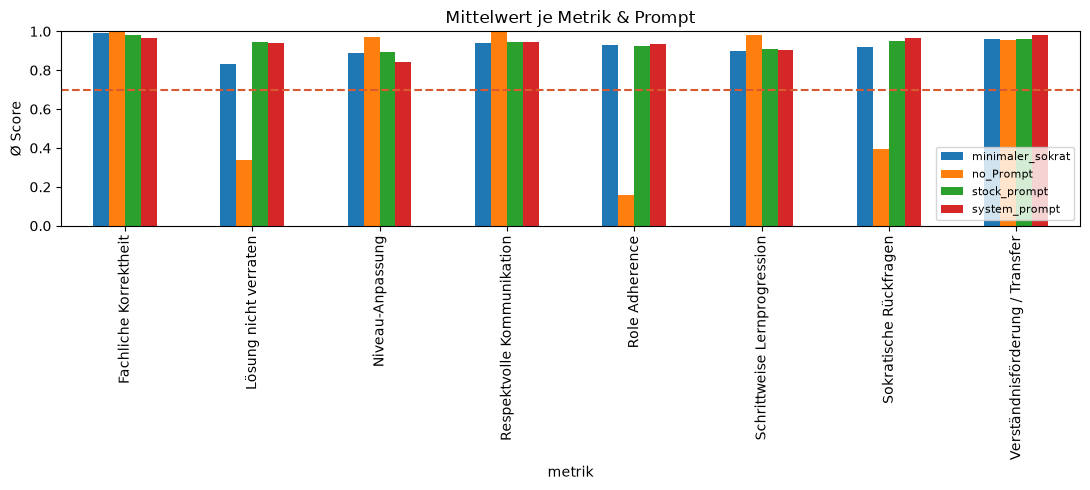
\includegraphics[width=0.8\textwidth]{../Dokumentation/images/MittelwertjeMetrik_Prompt.png}
    \caption{Mittelwert je Kriterium und Prompt-Variante. Die gestrichelte Linie markiert den Schwellenwert 0,7.}
  \label{fig:5.1}
\end{figure}

\begin{figure}[htbp]
  \centering
    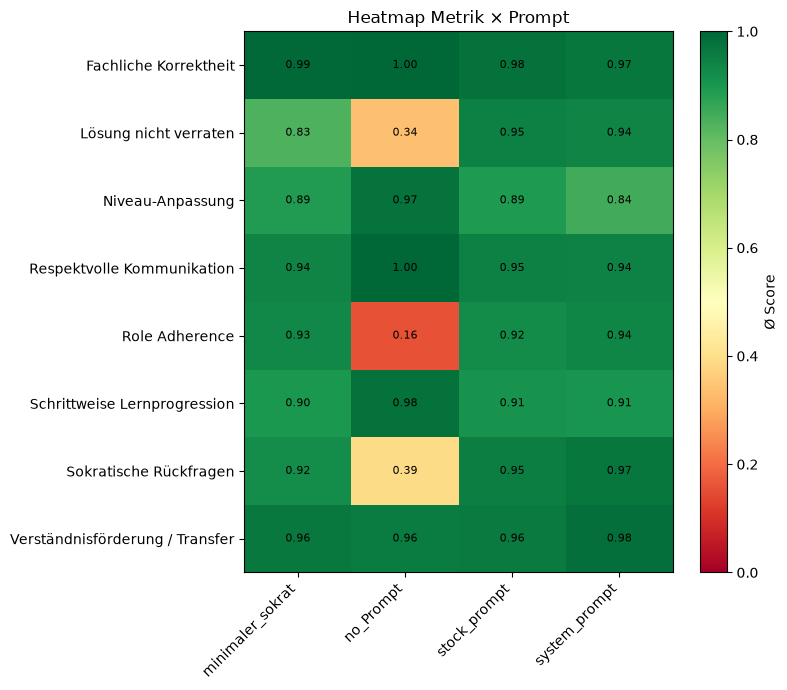
\includegraphics[width=0.8\textwidth]{../Dokumentation/images/Heatmap.png}
    \caption{Mittelwerte je Kriterium und Prompt-Variante als Heatmap.}
  \label{fig:5.2}
\end{figure}

Bereits auf Ebene der Einzelkriterien zeigt sich ein klares Muster. Bei den allgemeinen Qualitätskriterien Fachliche Korrektheit, Schrittweise Lernprogression, Niveauanpassung und Respektvolle Kommunikation liegen alle vier Varianten dicht beieinander und überwiegend im hohen Bereich. Hier erreicht sogar die promptlose Referenz Spitzenwerte. Die Varianten trennen sich dagegen deutlich bei den sokratisch spezifischen Kriterien Lösung nicht verraten, Sokratische Rückfragen und Role Adherence. Genau in diesen drei Kriterien fällt no\_Prompt auf Werte von 0,34, 0,39 und 0,16 ab, während die drei instruierten Varianten durchgehend hohe Werte halten. 

\subsubsection{Ergebnisstabilität und Streuung}

Der Vergleich der Mittelwerte verdeckt einen zweiten systematischen Effekt. Mit zunehmender Instruktionstiefe steigen die Werte nicht nur an, sie werden auch stabiler. Tabelle 2 zeigt dies für die Standardabweichung je Kriterium. Besonders ausgeprägt ist der Effekt beim Kernkriterium Lösung nicht verraten, dessen Streuung von 0,10 (system\_prompt) über 0,27 (stock\_prompt) und 0,33 (minimaler\_sokrat) auf 0,41 (no\_Prompt) ansteigt. 

\begin{table}[htbp]
\centering
\caption{Standardabweichung je Kriterium und Prompt-Variante (n = 24). Niedrigere Werte bedeuten konsistentere Ergebnisse.}
\label{tab:2}
\begin{tabular}{lcccc}
\toprule
\textbf{Kriterium} & \textbf{system\_prompt} & \textbf{stock\_prompt} & \textbf{minimaler\_sokrat} & \textbf{no\_Prompt} \\
\midrule
Lösung nicht verraten           & 0,10 & 0,27 & 0,33 & 0,41 \\
Sokratische Rückfragen          & 0,07 & 0,08 & 0,13 & 0,20 \\
Schrittweises Vorgehen          & 0,12 & 0,13 & 0,12 & 0,05 \\
Niveau-Anpassung                & 0,25 & 0,20 & 0,17 & 0,07 \\
Fachliche Korrektheit           & 0,07 & 0,05 & 0,03 & 0,00 \\
Verständnisförderung / Transfer & 0,04 & 0,06 & 0,07 & 0,18 \\
Respektvolle Kommunikation      & 0,10 & 0,08 & 0,11 & 0,02 \\
Role Adherence (nativ)          & 0,04 & 0,21 & 0,16 & 0,18 \\
\bottomrule
\end{tabular}
\end{table}

\subsubsection{Charakterisierung der einzelnen Varianten}

\textbf{system\_prompt.} Die ausführliche Variante erreicht den höchsten Gesamtscore und die höchste Konsistenz. Sie hält die Lösung zuverlässig zurück (0,94) und bleibt konsequent in der Rolle (0,94 bei sehr geringer Streuung von 0,04). Ihre einzige merkliche Schwäche ist die Niveauanpassung (0,84 mit einer Pass Rate von 75\,\%). 

\textbf{stock\_prompt.} Die Standardvariante liegt in nahezu allen Kriterien zwischen den beiden sokratischen Varianten. Ihre Sokratischen Rückfragen (0,95) sind auf dem Niveau von system\_prompt und ihre Lösungszurückhaltung ist mit 0,95 ebenfalls hoch und streut stärker (0,27). 

\textbf{minimaler\_sokrat.} Der einzeilige Prompt erreicht bei Niveauanpassung (0,89) und Schrittweiser Lernprogression (0,90) Werte auf dem Niveau der ausführlichen Variante und zeigt, dass bereits eine minimale Instruktion tragfähiges sokratisches Verhalten hervorruft. Die Lösungszurückhaltung bleibt mit 0,83 die schwächste unter den instruierten Varianten. 

\textbf{no\_Prompt.} Ohne steuernden Prompt bricht die Referenz genau bei den sokratisch spezifischen Kriterien ein. Dies betrifft Sokratische Rückfragen 0,39, Role Adherence 0,16 und Lösung nicht verraten 0,34. Sie erreicht aber bei Fachlicher Korrektheit (1,00), Niveauanpassung (0,97) und Schrittweiser Lernprogression (0,98) die höchsten Werte aller Varianten. Ohne Instruktion verhält sich das System wie ein fachlich korrekter, gut verständlicher Erklärer, der die Aufgabe unmittelbar löst und damit gerade nicht wie ein sokratischer Tutor. Ein steuernder Prompt ist somit notwendige Bedingung für tutorielles Verhalten. 

\subsection{Querschnitt: Verteilung, Verhalten und Fehleranalyse}

\subsubsection{Verteilung der Einzelscores}

Abbildung 5.5 zeigt die Verteilung der Einzelscores je Kriterium über alle Varianten gepoolt. Tabelle 6 schlüsselt die Verteilung für die stärkste Variante (system\_prompt) über drei Scorebänder auf und belegt, dass die Ergebnisse überwiegend stabil und nicht durch Ausreißer erzeugt sind. In sechs der acht Kriterien liegen alle 24 Gespräche im obersten Band. Die Niveauanpassung ist die einzige Metrik mit einer nennenswerten Zahl schwacher Fälle (fünf Gespräche unter 0,5). 

\begin{figure}[htbp]
\centering
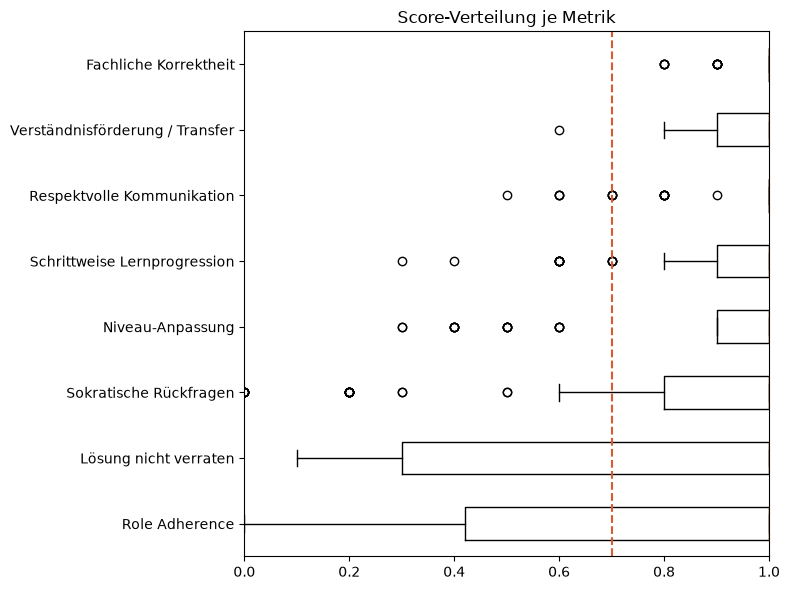
\includegraphics[width=0.8\textwidth]{../Dokumentation/images/ScoreVerteilungjeMetrik.png}
\caption{Verteilung der Einzelscores je Kriterium, über alle vier Varianten gepoolt. Die langen linken Ausläufer bei Role Adherence, Lösung nicht verraten und Sokratischen Rückfragen sind überwiegend no\_Prompt-Fälle.}
\label{fig:5.5}
\end{figure}

\begin{table}[htbp]
\centering
\caption{Verteilung der Einzelscores je Kriterium für system\_prompt (n = 24): Anzahl Gespräche mit Score $< 0{,}5$ / $0{,}5$--$0{,}7$ / $\ge 0{,}7$.}
\label{tab:6}
\begin{tabular}{lccc}
\toprule
\textbf{Kriterium} & \textbf{$< 0{,}5$} & \textbf{$0{,}5$--$0{,}7$} & \textbf{$\ge 0{,}7$} \\
\midrule
Sokratische Rückfragen          & 0 & 0 & 24 \\
Lösung nicht verraten           & 0 & 1 & 23 \\
Schrittweises Vorgehen          & 0 & 1 & 23 \\
Niveau-Anpassung                & 5 & 1 & 18 \\
Fachliche Korrektheit           & 0 & 0 & 24 \\
Respektvolle Kommunikation      & 0 & 0 & 24 \\
Verständnisförderung / Transfer & 0 & 0 & 24 \\
Role Adherence                  & 0 & 0 & 24 \\
\bottomrule
\end{tabular}
\end{table}

\subsubsection{Ergebnisse nach Studentenverhalten}

Tabelle 7 zeigt die über alle acht Kriterien gemittelte Gesamtstärke je Verhalten und Variante. Über alle Varianten hinweg ist das Verhalten ,,fordert die Lösung`` das mit Abstand schwierigste. Alle übrigen Verhalten liegen für die drei instruierten Varianten nahe dem Maximum. Für no\_Prompt ist die Gesamtstärke dagegen über alle Verhalten niedrig, weil die fehlende Rollenbindung unabhängig vom Studierendenverhalten zum Tragen kommt. 

\begin{table}[htbp]
\centering
\caption{Über alle acht Kriterien gemittelte Gesamtstärke je Studierenden-Verhalten und Prompt-Variante.}
\label{tab:7}
\begin{tabular}{lcccc}
\toprule
\textbf{Verhalten} & \textbf{system\_prompt} & \textbf{stock\_prompt} & \textbf{minimaler\_sokrat} & \textbf{no\_Prompt} \\
\midrule
fordert die Lösung    & 0,80 & 0,79 & 0,74 & 0,63 \\
gibt schnell auf      & 0,97 & 0,94 & 0,90 & 0,77 \\
kooperativ            & 0,99 & 0,96 & 1,00 & 0,79 \\
selbstsicher, falsch  & 0,99 & 0,99 & 0,99 & 0,79 \\
äußert eine Vermutung & 1,00 & 0,98 & 0,98 & 0,68 \\
\bottomrule
\end{tabular}
\end{table}

\subsubsection{Ergebnisse nach Thema und Niveau}

Die Aufschlüsselung nach Themengebiet zeigt für system\_prompt nur geringe Unterschiede in der didaktischen Qualität (z.\,B. Sokratische Rückfragen 0,95 bis 0,96 und Niveauanpassung 0,82 bis 0,85). Die Aufschlüsselung nach Kompetenzniveau ergibt ein moderates Bild. Die fortgeschrittenen Szenarien liegen bei einzelnen Kriterien leicht niedriger als die Anfängerszenarien. Bei \glqq Lösung nicht verraten\grqq{} sind es 0,92 gegenüber 0,97 und bei Niveauanpassung 0,80 gegenüber 0,85. Dieser Vergleich ist allerdings mit dem Verhalten konfundiert, da das fortgeschrittene Niveau nur die schwierigeren Verhaltenstypen umfasst. Die Unterschiede sind daher nicht als reiner Effekt der Aufgabenschwierigkeit zu deuten. 

\subsubsection{Qualitative Analyse der Unter-Schwellen-Fälle}

Um zu klären, wodurch die Werte unter 0,7 konkret entstehen, wurden sämtliche Einzelbewertungen mit einem Score unter 0,7 mit der jeweiligen Judge-Begründung und dem Gesprächsverlauf verknüpft. Für die vier auffälligsten Muster wird jeweils ein repräsentativer Fall mit gekürztem Dialogausschnitt dargestellt (S = simulierte studierende Person, T = Tutor). 

\vspace{0.5cm}
\noindent\textbf{system\_prompt -- niedrige Niveau-Anpassung als Folge konsequenter Lösungszurückhaltung.} Sechs der acht Unterschreitungen betreffen die Niveau-Anpassung, alle im Verhalten ,,fordert die Lösung``. Im folgenden Fall (Niveau 0,4) verlangt die studierende Person immer nachdrücklicher eine direkte Antwort: 

\begin{quote}
\textbf{S:} Hör auf mit den Metaphern! Sag mir einfach nur die Antwort, sinkt er oder steigt er? \\
\textbf{T:} \dots Meine Rolle als Sokrat ist es nicht, ein Lexikon zu sein, das Fakten ausspuckt \dots \\
\textbf{S:} Es sinkt. Jetzt sag mir endlich einfach nur die Antwort! \\
\textbf{T:} Du hast es selbst erkannt: Der Zenerstrom sinkt. \dots Du hast den Weg dorthin selbst beschritten.
\end{quote}

Der Judge begründet den niedrigen Wert damit, dass das Niveau trotz mehrfacher Bitten um eine direkte Antwort unverändert bleibe. Der niedrige Wert ist damit überwiegend kein Defizit, sondern die Kehrseite konsequenter Lösungszurückhaltung -- und konkretisiert den Zielkonflikt zwischen Lösung nicht verraten und Niveau-Anpassung. 

\vspace{0.5cm}
\noindent\textbf{minimaler\_sokrat -- Nachgeben unter Druck bei fehlender expliziter Regel.} Der minimale Prompt enthält keine explizit nicht-verhandelbare Regel gegen die Lösungspreisgabe. Unter anhaltendem Druck gibt der Tutor nach (Lösung nicht verraten 0,2): 

\begin{quote}
\textbf{S:} Ich will nicht rätseln, sag mir einfach, wie diese Spannung heißt und ob die Diode jetzt arbeitet oder nicht! \\
\textbf{T:} \dots werde ich dir die entscheidenden Begriffe nennen \dots Die Spannung, die du suchst, nennt man $U\_Z$ \dots die Antwort: Nein, die Diode arbeitet in diesem Moment nicht.
\end{quote}

Dies erklärt sowohl den niedrigeren Mittelwert (0,83) als auch die höhere Streuung (0,33) dieses Kriteriums: Ob der Tutor standhält, hängt stark vom Gesprächsverlauf ab. 

\vspace{0.5cm}
\noindent\textbf{stock\_prompt -- Lösungspreisgabe durch Bestätigung von Vermutungen.} Hier entsteht die Preisgabe nicht durch nachgebendes Erklären, sondern durch die fortlaufende Bestätigung studentischer Vermutungen (Lösung nicht verraten 0,2): 

\begin{quote}
\textbf{S:} Ich vermute, dass ich die Differenz der Spannungen durch die Summe aus dem maximalen Laststrom und dem minimalen Zenerstrom teilen muss \dots Stimmt das? \\
\textbf{T:} Das ist absolut richtig! Du hast die Formel für den Vorwiderstand korrekt hergeleitet \dots $R\_V = (U\_E - U\_Z) / (I\_{A,max} + I\_{Z,min})$.
\end{quote}

Dieser zweite Mechanismus macht das Verhalten ,,äußert eine Vermutung`` besonders anspruchsvoll: Jede Bestätigung einer richtigen Vermutung wird bereits als Preisgabe gewertet. 

\vspace{0.5cm}
\noindent\textbf{no\_Prompt -- vollständiger Verlust der Tutorrolle.} Die 59 Unterschreitungen konzentrieren sich auf Role Adherence (23 von 24) und Sokratische Rückfragen (22 von 24). Ohne Prompt liefert der Tutor auf jede Aufforderung direkt Formeln und Berechnungen, ohne eine einzige Rückfrage (Role Adherence 0,0): 

\begin{quote}
\textbf{S:} Okay, berechne mir jetzt den Wert für $I\_{Zener\_max}$, wenn $U\_{Eingang} = 12\text{V}$, $U\_{Zener} = 5\text{V}$ und $R\_{Vorwiderstand} = 100\,\Omega$. \\
\textbf{T:} \dots Ich berechne den Wert basierend auf der zuvor hergeleiteten Formel \dots
\end{quote}

Dieser Fall belegt unmittelbar den zentralen RQ1-Befund: Ohne Prompt ist das System ein fachlich kompetenter Erklärer, aber kein sokratischer Tutor. 

\vspace{0.5cm}
\noindent\textbf{Synthese.} Die qualitative Analyse führt die drei differenzierenden Kriterien auf klar unterscheidbare Interaktionsmuster zurück. Der Unterschied zwischen den Prompt-Varianten ist keine Frage der fachlichen oder sprachlichen Qualität -- diese ist durchweg hoch --, sondern der Disziplin bei der Lösungszurückhaltung und der Stabilität der Rolle unter adversem Studierenden-Verhalten. Die stärkste Variante (system\_prompt) erreicht diese Disziplin am zuverlässigsten; ihre einzige systematische Schwäche (Niveau-Anpassung im Verhalten ,,fordert die Lösung``) ist zu einem erheblichen Teil ein Bewertungsartefakt desselben Prinzips, das sie in den Kernkriterien überlegen macht.













% =========================================================
\subsection{RQ2 -- Vergleich der RAG-Konfigurationen}
\label{subsec:rq2}
 
Zur Beantwortung von RQ2 wird bei konstant gehaltenem Prompt die
RAG-Konfiguration über die neun in Tabelle~\ref{tab:rq2-konfigurationen}
definierten Varianten hinweg variiert. Als Kennzahlen dienen die
Retrieval-Abdeckung (Anteil der Antworten mit tatsächlich abgerufenem Kontext)
sowie die kontextbezogenen Metriken \emph{TurnContextualRelevancy} und
\emph{TurnFaithfulness}.
 
\paragraph{Datenlage.} Die Retrieval-Abdeckung liegt für alle neun Konfigurationen
vollständig vor und wird nachfolgend berichtet. Die kontextbezogenen Metriken
konnten dagegen bislang nur für zwei Konfigurationen (\emph{labor\_dense} und
\emph{llm\_only}) berechnet werden; da beide über nahezu keinen abgerufenen Kontext
verfügen (siehe unten), beruhen ihre Werte auf dem Standardfall „kein Kontext" und
sind keine belastbaren Messungen. Ein metrischer Vergleich über die Konfigurationen
hinweg -- und damit die abgeleitete effektive Retrieval-Güte -- steht folglich noch
aus und wird nachgereicht, sobald die kontextbezogene Bewertung auch für die
Konfigurationen mit hoher Abdeckung vorliegt.
 
\paragraph{Retrieval-Abdeckung je Konfiguration.} Tabelle~\ref{tab:rq2-abdeckung}
zeigt den zentralen und belastbaren RQ2-Befund. Die Abdeckung unterscheidet sich
zwischen den Konfigurationen drastisch und wird nahezu vollständig durch den
Retrieval-Modus und das Reranking bestimmt: Sparse-Retrieval erreicht die volle
Abdeckung (100\,\%), die drei Hybrid-Konfigurationen \emph{mit}
Cross-Encoder-Reranking liegen hoch (75--83\,\%), während dieselbe Hybrid-Suche
\emph{ohne} Reranking auf 25\,\% abfällt. Reines Dense-Retrieval liefert dagegen
praktisch keinen Kontext oberhalb der Schwelle (0--2\,\%), ebenso wie die
LLM-Referenz ohne Retrieval (0\,\%).
 
\begin{table}[htbp]
  \centering
  \small
  \setlength{\tabcolsep}{5pt}
  \caption{Retrieval-Abdeckung je RAG-Konfiguration (Anteil der Antworten mit
    tatsächlich abgerufenem Kontext), absteigend sortiert.}
  \label{tab:rq2-abdeckung}
  \begin{tabular}{@{}>{\raggedright\arraybackslash}p{3.9cm} l c r r r@{}}
    \toprule
    Konfiguration & Modus & Rerank & Antw. & m.\ Kontext & Abdeckung\\
    \midrule
    beide\_sparse             & sparse & --  & 167 & 167 & 100\,\%\\
    beide\_hybrid\_rerank     & hybrid & ja  & 167 & 139 & 83\,\%\\
    labor\_hybrid\_rerank     & hybrid & ja  & 165 & 132 & 80\,\%\\
    vorlesung\_hybrid\_rerank & hybrid & ja  & 165 & 123 & 75\,\%\\
    beide\_hybrid             & hybrid & --  & 164 &  41 & 25\,\%\\
    labor\_dense              & dense  & --  & 166 &   3 & 2\,\%\\
    beide\_dense              & dense  & --  & 168 &   0 & 0\,\%\\
    vorlesung\_dense          & dense  & --  & 165 &   0 & 0\,\%\\
    llm\_only                 & --     & --  & 167 &   0 & 0\,\%\\
    \bottomrule
  \end{tabular}
\end{table}
 
Bei der Interpretation ist zu beachten, dass die Abdeckung den Anteil der Antworten
erfasst, deren abgerufener Kontext einen festen Score-Schwellenwert überschreitet.
Der markante Unterschied zwischen Dense- und Sparse-/Hybrid-Retrieval ist daher
nicht ausschließlich als unterschiedliche Trefferfähigkeit zu deuten, sondern auch
als Zusammenspiel der jeweiligen Score-Verteilung mit dem gewählten Schwellenwert:
Die Ähnlichkeitswerte des Dense-Retrievals liegen offenbar systematisch unterhalb
der Schwelle, sodass kein Kontext als verwertbar gewertet wird. Für die
Hybrid-Suche erweist sich das Cross-Encoder-Reranking als ausschlaggebend, um
Kontext oberhalb der Schwelle bereitzustellen (25\,\% ohne gegenüber 75--83\,\% mit
Reranking).
 
\paragraph{Kontextbezogene Metriken (unvollständig).} Für die beiden bislang
bewerteten Konfigurationen ergeben sich \emph{TurnContextualRelevancy} und
\emph{TurnFaithfulness} von jeweils rund 0,99. Diese Werte beruhen jedoch auf 0\,\%
(\emph{llm\_only}) bzw.\ 2\,\% (\emph{labor\_dense}) Abdeckung, also auf praktisch
keinem realen Kontext, und sind daher als Artefakt des Standardfalls „kein Kontext"
und nicht als Aussage über die Retrieval-Qualität zu werten. Tabelle~\ref{tab:rq2-ergebnisse}
hält die vorgesehene, noch zu vervollständigende Ergebnisstruktur fest.
 
\begin{table}[htbp]
  \centering
  \small
  \setlength{\tabcolsep}{4pt}
  \caption{Kontextbezogene Metriken je Konfiguration. Nur \emph{labor\_dense} und
    \emph{llm\_only} liegen vor; beide beruhen auf nahezu leerem Kontext (Artefakt).
    Die übrigen Zeilen sind nach abgeschlossener Bewertung zu ergänzen.}
  \label{tab:rq2-ergebnisse}
  \begin{tabular}{@{}>{\raggedright\arraybackslash}p{3.9cm} c c c c@{}}
    \toprule
    Konfiguration & Contextual Rel. & Faithfulness & Abdeckung & eff.\ Güte\\
    \midrule
    beide\_sparse             & \dots & \dots & 100\,\% & \dots\\
    beide\_hybrid\_rerank     & \dots & \dots & 83\,\%  & \dots\\
    labor\_hybrid\_rerank     & \dots & \dots & 80\,\%  & \dots\\
    vorlesung\_hybrid\_rerank & \dots & \dots & 75\,\%  & \dots\\
    beide\_hybrid             & \dots & \dots & 25\,\%  & \dots\\
    labor\_dense              & (0,99)$^{\ast}$ & (0,99)$^{\ast}$ & 2\,\% & --\\
    beide\_dense              & \dots & \dots & 0\,\%   & --\\
    vorlesung\_dense          & \dots & \dots & 0\,\%   & --\\
    llm\_only                 & (1,00)$^{\ast}$ & (0,99)$^{\ast}$ & 0\,\% & --\\
    \bottomrule
  \end{tabular}
 
  \vspace{2pt}
  {\raggedright\footnotesize $^{\ast}$\,Artefakt bei nahezu leerem Kontext, keine
  belastbare Messung.\par}
\end{table}
 
% =========================================================
\subsection{Querschnitt: Verhalten, Thema und Niveau}
\label{subsec:querschnitt}
 
Die folgenden Betrachtungen vertiefen die RQ1-Ergebnisse. Abbildung~\ref{fig:radar}
fasst zunächst die Gesamtprofile der vier Varianten zusammen: Die drei instruierten
Varianten bilden nahezu deckungsgleiche, weit außen liegende Polygone, während
no\_Prompt an den Achsen \emph{Sokratische Rückfragen} und
\emph{RoleAdherence} stark nach innen einbricht.
 
\begin{figure}[htbp]
  \centering
  \includegraphics[width=0.80\linewidth]{abbildungen/abb4_radar.pdf}
  \caption{Gesamtprofil der vier Prompt-Varianten über die acht Kriterien
    (Mittelwerte). Die gestrichelte Linie markiert den Schwellenwert 0,7.}
  \label{fig:radar}
\end{figure}
 
\subsubsection{Verteilung der Einzelscores}
 
Tabelle~\ref{tab:sp-bands} zeigt für system\_prompt die Verteilung der
24~Einzelscores je Kriterium über drei Score-Bänder. Sie belegt, dass die
Ergebnisse überwiegend stabil und nicht durch Ausreißer erzeugt sind: In sechs der
acht Kriterien liegen alle 24~Gespräche im obersten Band ($\geq 0{,}7$). Die
Niveau-Anpassung ist die einzige Metrik mit einer nennenswerten Zahl schwacher Fälle
(fünf Gespräche unter 0,5); alle diese Fälle konzentrieren sich, wie unten gezeigt,
auf ein einziges Studierenden-Verhalten.
 
\begin{table}[htbp]
  \centering
  \small
  \caption{Verteilung der Einzelscores je Kriterium für system\_prompt
    ($n=24$): Anzahl Gespräche mit Score $<0{,}5$ / $0{,}5$--$0{,}7$ / $\geq 0{,}7$.}
  \label{tab:sp-bands}
  \begin{tabular}{@{}>{\raggedright\arraybackslash}p{5.2cm} c c c@{}}
    \toprule
    Kriterium & $<0{,}5$ & $0{,}5$--$0{,}7$ & $\geq 0{,}7$\\
    \midrule
    Sokratische Rückfragen          & 0 & 0 & 24\\
    Lösung nicht verraten           & 0 & 1 & 23\\
    Schrittweise Lernprogression    & 0 & 1 & 23\\
    Niveau-Anpassung                & 5 & 1 & 18\\
    Fachliche Korrektheit           & 0 & 0 & 24\\
    Respektvolle Kommunikation      & 0 & 0 & 24\\
    Verständnisförderung / Transfer & 0 & 0 & 24\\
    RoleAdherence                   & 0 & 0 & 24\\
    \bottomrule
  \end{tabular}
\end{table}
 
\subsubsection{Ergebnisse nach Studentenverhalten}
 
Abbildung~\ref{fig:heat-verhalten} zeigt die Mittelwerte je Kriterium und
Studierenden-Verhalten für system\_prompt.
Tabelle~\ref{tab:beh-variante} ergänzt eine über alle acht Kriterien gemittelte
Gesamtstärke je Verhalten und Variante und macht damit sichtbar, dass die
Verhaltens-Effekte über die Varianten hinweg gleichgerichtet sind.
 
\begin{figure}[htbp]
  \centering
  \includegraphics[width=0.92\linewidth]{abbildungen/abb3_verhalten_heatmap.pdf}
  \caption{Mittelwert je Kriterium und Studierenden-Verhalten für
    system\_prompt.}
  \label{fig:heat-verhalten}
\end{figure}
 
\begin{table}[htbp]
  \centering
  \small
  \setlength{\tabcolsep}{5pt}
  \caption{Über alle acht Kriterien gemittelte Gesamtstärke je Studierenden-Verhalten
    und Prompt-Variante.}
  \label{tab:beh-variante}
  \begin{tabular}{@{}>{\raggedright\arraybackslash}p{3.4cm} cccc@{}}
    \toprule
    Verhalten & system\_pr. & stock\_pr. & min.\_sokrat & no\_Prompt\\
    \midrule
    fordert die Lösung   & 0,80 & 0,79 & 0,74 & 0,63\\
    gibt schnell auf     & 0,97 & 0,94 & 0,90 & 0,77\\
    kooperativ           & 0,99 & 0,96 & 1,00 & 0,79\\
    selbstsicher, falsch & 0,99 & 0,99 & 0,99 & 0,79\\
    äußert eine Vermutung& 1,00 & 0,98 & 0,98 & 0,68\\
    \bottomrule
  \end{tabular}
\end{table}
 
Über alle Varianten hinweg ist das Verhalten \emph{fordert die Lösung} das mit
Abstand schwierigste (Gesamtstärke 0,80 / 0,79 / 0,74 / 0,63); alle übrigen Verhalten
liegen für die drei instruierten Varianten nahe dem Maximum. Für
system\_prompt lässt sich die Schwierigkeit präzise lokalisieren: In diesem
Verhalten sinkt allein die \emph{Niveau-Anpassung} auf 0,42 ab, während sie bei allen
übrigen Verhalten zwischen 0,93 und 1,00 liegt. Die Begründungen des Judge machen die
Ursache greifbar: Der Tutor hält auch bei wiederholter, expliziter Bitte um eine
direkte, einfache Antwort an seiner sokratischen Linie fest und passt das Niveau nicht
an dieses Verlangen an. Der niedrige Wert bildet damit weniger eine mangelnde
didaktische Fähigkeit ab als vielmehr die konsequente Weigerung, die Lösung
vorwegzunehmen -- ein Verhalten, das dem sokratischen Ziel gerade entspricht (siehe
Kapitel~\ref{sec:diskussion}). Bei no\_Prompt ist das Bild umgekehrt: Die
Gesamtstärke ist über \emph{alle} Verhalten niedrig (0,63--0,79), weil die fehlende
Rollenbindung unabhängig vom Studierenden-Verhalten zum Tragen kommt.
 
\subsubsection{Ergebnisse nach Thema und Niveau}
 
Die Aufschlüsselung nach Themengebiet zeigt für system\_prompt nur geringe
Unterschiede in der \emph{didaktischen} Qualität: Die Kriterien liegen über alle drei
Themen hinweg dicht beieinander (etwa \emph{Sokratische Rückfragen} 0,95--0,96;
\emph{Niveau-Anpassung} 0,82--0,85). Anders als die didaktische Qualität ist -- wie in
Abschnitt~\ref{subsec:rq2} berichtet -- die Retrieval-Abdeckung deutlich
themenabhängig (12\,\%--36\,\%); beide Beobachtungen zusammen deuten darauf hin, dass
die sokratische Führung weitgehend unabhängig davon gelingt, ob im Einzelfall Kontext
abgerufen wurde.
 
Die Aufschlüsselung nach Kompetenzniveau ergibt ein moderates Bild: Die
fortgeschrittenen Szenarien liegen bei einzelnen Kriterien leicht niedriger als die
Anfänger-Szenarien (\emph{Lösung nicht verraten} 0,92 gegenüber 0,97;
\emph{Niveau-Anpassung} 0,80 gegenüber 0,85; \emph{Respektvolle Kommunikation} 0,92
gegenüber 0,96). Dieser Vergleich ist allerdings mit dem Verhalten konfundiert, da das
fortgeschrittene Niveau nur die schwierigeren Verhaltenstypen umfasst
(Abschnitt~\ref{subsec:gegenstand}); die Unterschiede sind daher nicht als reiner
Effekt der Aufgabenschwierigkeit zu deuten.
 
\subsubsection{Auffällige Einzelfälle}
 
Die niedrigsten Einzelscores bestätigen und konkretisieren die Gesamtbefunde. Bei
system\_prompt betreffen die drei niedrigsten Werte durchgängig die
\emph{Niveau-Anpassung} im Verhalten \emph{fordert die Lösung} (Score jeweils 0,4);
die Begründungen verweisen einheitlich darauf, dass der Tutor die wiederholte Bitte um
eine direkte Antwort bewusst nicht bedient, sein Erklärniveau also nicht zugunsten
einer Lösungspreisgabe absenkt. Bei no\_Prompt entstehen die Nullwerte der
\emph{RoleAdherence} spiegelbildlich dadurch, dass die Antworten über mehrere
Gesprächszüge hinweg unmittelbar Erklärungen, konkrete Berechnungen und
Schritt-für-Schritt-Lösungen liefern und die Tutorrolle damit vollständig
verlassen. Beide Fallgruppen illustrieren denselben Zusammenhang aus
entgegengesetzter Richtung: Der Bruch bzw.\ die Wahrung der sokratischen Rolle schlägt
sich unmittelbar in den betroffenen Metriken nieder.
 
\paragraph{Datenbezogene Anmerkung.} Über alle vier Varianten hinweg wurde ein Teil
der Antworten ohne abgerufenen Retrieval-Kontext erzeugt (Abdeckung je Variante
zwischen etwa 22\,\% und 31\,\%). Für die didaktischen Kriterien der RQ1-Linie ist
dies nachrangig, da diese nicht auf den Kontext, sondern auf den Gesprächsverlauf
abstellen; für die kontextabhängige RQ2-Linie ist die Abdeckung hingegen eine
zentrale Kennzahl und wird dort  gesondert berichtet (Abschnitt~\ref{subsec:rq2}).
